\documentclass[11pt,a4paper]{article}
\usepackage[T1]{fontenc}
\usepackage[margin=2.3cm]{geometry}
\usepackage{amsmath,amssymb}
\usepackage{graphicx}
\usepackage[dvipsnames]{xcolor}
\usepackage{enumitem}
\usepackage[colorlinks=true,linkcolor=blue,urlcolor=blue]{hyperref}
\setlength{\parskip}{0.6em}
\setlength{\parindent}{0pt}
\begin{document}

\begin{center}{\LARGE\bfseries openbuoyancy}\\[0.4em]{\large Will it float, and will it stay upright? Archimedes in three sessions.}\\[0.2em]\small PAN IIT OSS explainer \textbullet{} higher secondary to diploma / undergraduate (levels 4-5)\end{center}

\section*{Why this exists}
Every ship, raft and balloon floats because of one idea of Archimedes, and every ship stays upright or rolls over because of where its weight sits relative to its metacentre. This explainer shows the mathematics with a box-shaped barge, so you can build it yourself.

\section*{The end goal}
Decide whether a ship floats and stays upright using Archimedes' principle. The end goal is to decide whether a vessel floats and stays upright using Archimedes' principle. The same reasoning is behind life jackets, submarines, hot-air balloons and the loading rules for real ships, although those use far more detailed methods than this teaching model.

\section*{How the three sessions build up}
\begin{enumerate}[nosep]
\item \textbf{Session 1: Things float when the water they push aside weighs as much as they do} (Level 1, conceptual interactive model, 60 min).
\item \textbf{Session 2: The buoyant force, barge loads and balloon lift} (Level 2, mathematical engineering model, 75 min).
\item \textbf{Session 3: Does it stay upright? Metacentric height and the righting arm} (Level 3, simulation and validation, 90 min).
\end{enumerate}

\section{Session 1: Things float when the water they push aside weighs as much as they do}

\subsection*{A. Real-world problem}
A steel ship weighs thousands of tonnes and floats. A pebble weighs a few grams and sinks. A wooden block floats low in a pond and a little higher in the sea. Why? Can you predict, before you try, whether something floats and how deep it will sit? (This is general science education, not a guide for boat safety.)

\subsection*{B. Concept and theory}
When an object is lowered into water it pushes some water out of its way. The water pushes back with a force equal to the weight of the water that was pushed aside (Archimedes' principle). An object floats when it can push aside its own weight in water before it is fully under. Because water displaced = fluid density times submerged volume, an object floats when its average density (total mass divided by total outside volume, including any air inside) is below the fluid's density, and then a fraction rho\_object / rho\_fluid of its volume is below the surface. For a flat-bottomed box with bottom area A, the depth under water (the draft) is mass / (rho\_fluid * A). A hollow steel boat floats because its average density includes the air inside.

\begin{itemize}[nosep]
\item rho\_obj: average density of the object (mass / outside volume) (kg/m\textasciicircum{}3)
\item rho\_fluid: density of the fluid (fresh water 1000, sea water about 1025) (kg/m\textasciicircum{}3)
\item f: fraction of the object's volume under water (no unit)
\item m: mass of the object (kg)
\item A: area of the flat bottom (m\textasciicircum{}2)
\item draft: depth of the bottom below the water line (m)
\end{itemize}

\begin{equation*}
\rho_{obj}=\frac{m}{V}
\end{equation*}

\begin{equation*}
f=\min\!\left(1,\ \frac{\rho_{obj}}{\rho_{fluid}}\right)
\end{equation*}

\begin{equation*}
\text{draft}=\frac{m}{\rho_{fluid}\,A}
\end{equation*}

\begin{center}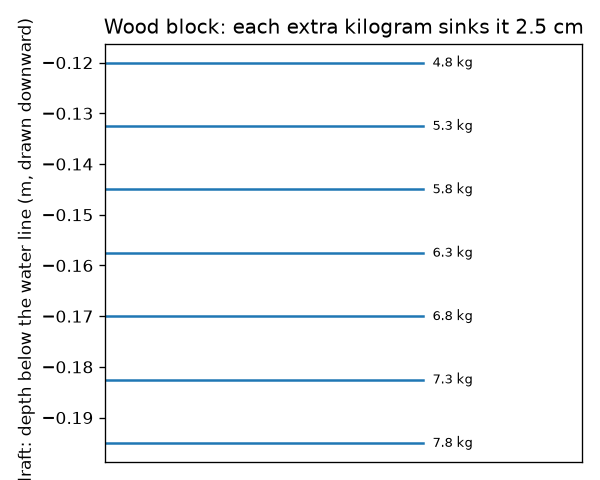
\includegraphics[width=0.85\linewidth]{figures/s01_draft_marks.png}\\\small Draft marks of a wooden block: each extra kilogram adds 2.5 cm of draft.\end{center}

\subsection*{E. Worked example}
A wooden cube of side 0.2 m has mass 4.8 kg. Does it float in fresh water? How deep does it sit? What happens in sea water (1025 kg/m\textasciicircum{}3)?
\begin{enumerate}[nosep]
\item Volume = 0.2 * 0.2 * 0.2 = 0.008 m\textasciicircum{}3, so average density = 4.8 / 0.008 = 600 kg/m\textasciicircum{}3.
\item 600 is below 1000, so it floats. Fraction under water = 600 / 1000 = 0.60.
\item Bottom area = 0.2 * 0.2 = 0.04 m\textasciicircum{}2, so draft = 4.8 / (1000 * 0.04) = 0.120 m (60 percent of 0.2 m, as it must be).
\item In sea water: draft = 4.8 / (1025 * 0.04) = 0.117 m. It sits about 3 mm higher.
\end{enumerate}
\textbf{Answer.} It floats with 60 percent under water, draft 0.120 m in fresh water and 0.117 m in sea water.

\subsection*{F. Questions}
\begin{enumerate}[nosep]
\item \textbf{Conceptual.} Steel has a density of about 7850 kg/m\textasciicircum{}3, yet a steel ship floats. Explain, and say what would happen to the same steel hammered into a solid lump.
\item \textbf{Numerical.} A block of mass 2.0 kg has a volume of 0.0030 m\textasciicircum{}3. Find its average density, whether it floats in fresh water, the fraction under water and the mass of water it pushes aside.
\item \textbf{Graph and simulation interpretation.} In the graph of submerged fraction against density, the line stops rising at density 1000 (fresh water). What does an object of density 1010 kg/m\textasciicircum{}3 do in fresh water and in sea water?
\item \textbf{Design and optimisation challenge.} Design: a flat-bottomed boat has an empty mass of 150 kg and a bottom of 2.0 m by 0.8 m. In calm fresh water it must keep a draft of no more than 0.25 m. What is the largest cargo? State your assumptions.
\end{enumerate}

\section{Session 2: The buoyant force, barge loads and balloon lift}

\subsection*{A. Real-world problem}
A river barge is 20 m long and 6 m wide. How much cargo can it carry before its deck goes under water? Does the answer change when it sails out to sea? And how can a balloon rise in air with the same law? (Educational model: real vessels need larger margins, rules and professional design.)

\subsection*{B. Concept and theory}
The buoyant force on a body equals the weight of the fluid it displaces: F\_b = rho\_fluid g V\_displaced. A body floats in equilibrium when this equals its weight m g. For a rectangular barge of length L, beam B and hull depth H, the displaced volume is L B d, so the draft is d = m / (rho L B) and the freeboard (deck height above the water) is H - d. The deck reaches the water at d = H, so the greatest total mass is rho L B H, and the load capacity is that minus the empty (lightship) mass; designers keep a minimum freeboard f\_min, which lowers it to rho L B (H - f\_min) - m\_lightship. Air is also a fluid: a balloon filled with a gas of density rho\_gas in air of density rho\_air experiences a net lift of (rho\_air - rho\_gas) g V, so the lift per cubic metre is the density difference. The density of an ideal gas is rho = P M / (R T).

\begin{itemize}[nosep]
\item F\_b: buoyant force (N)
\item rho: density of the fluid (kg/m\textasciicircum{}3)
\item g: gravity, 9.81 (m/s\textasciicircum{}2)
\item V: displaced volume (m\textasciicircum{}3)
\item L, B, H: barge length, beam (width), hull depth (m)
\item d: draft (m)
\item m: total mass of barge and cargo (kg)
\item P, M, R, T: gas pressure (Pa), molar mass (kg/mol), gas constant 8.314 J/(mol K), temperature (K) (as stated)
\end{itemize}

\begin{equation*}
F_b=\rho_{fluid}\,g\,V_{displaced}
\end{equation*}

\begin{equation*}
d=\frac{m}{\rho\,L\,B}\qquad \text{freeboard}=H-d
\end{equation*}

\begin{equation*}
m_{cargo,max}=\rho\,L\,B\,(H-f_{min})-m_{lightship}
\end{equation*}

\begin{equation*}
\text{lift per m}^3=\rho_{air}-\rho_{gas}\ \ (\mathrm{kg/m^3}),\qquad \rho=\frac{P\,M}{R\,T}
\end{equation*}

\begin{center}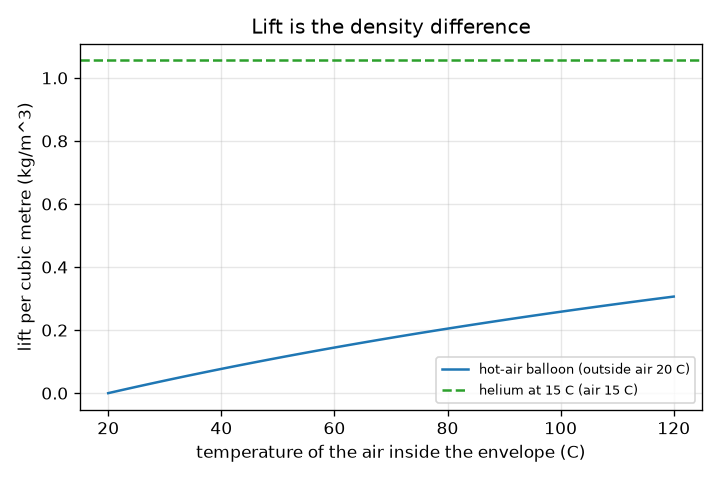
\includegraphics[width=0.85\linewidth]{figures/s02_balloon_lift.png}\\\small Lift per cubic metre of a hot-air balloon against the inside temperature, with helium for comparison.\end{center}

\subsection*{E. Worked example}
A barge 20 m long, 6 m wide with hull depth 2.5 m and empty mass 60 t carries 100 t in fresh water. Find the draft and freeboard, the greatest cargo with the deck just awash, and the greatest cargo if 0.3 m of freeboard must remain.
\begin{enumerate}[nosep]
\item Total mass = 60 000 + 100 000 = 160 000 kg. Draft = 160 000 / (1000 * 20 * 6) = 1.333 m.
\item Freeboard = 2.5 - 1.333 = 1.167 m.
\item Deck awash: greatest total mass = 1000 * 20 * 6 * 2.5 = 300 000 kg, so cargo = 300 000 - 60 000 = 240 000 kg = 240 t.
\item With 0.3 m freeboard: 1000 * 20 * 6 * (2.5 - 0.3) = 264 000 kg total, so cargo = 204 t.
\item Check with the buoyant force: at 1.333 m draft the displaced volume is 160 m\textasciicircum{}3 and F\_b = 1000 * 9.81 * 160 = 1.57 MN, equal to the weight 160 000 * 9.81 N.
\end{enumerate}
\textbf{Answer.} Draft 1.333 m, freeboard 1.167 m, capacity 240 t with the deck awash and 204 t with 0.3 m freeboard.

\subsection*{F. Questions}
\begin{enumerate}[nosep]
\item \textbf{Conceptual.} The barge sails from a river into the sea. Does its draft increase or decrease, and by what fraction? Why is this still true if the barge is empty?
\item \textbf{Numerical.} The same barge (20 x 6 x 2.5 m, empty 60 t) carries 100 t of cargo in sea water. Find the draft.
\item \textbf{Graph and simulation interpretation.} In the draft graph, the sea-water line meets the red deck line at a larger cargo than the fresh-water line. Read both values and say what the difference means.
\item \textbf{Design and optimisation challenge.} Design: a raft is 3.0 m long, 0.25 m deep and has a mass of 10 kg per square metre of deck. It must carry 15 people of 65 kg in fresh water and keep a freeboard of at least 0.10 m. What is the narrowest width, in steps of 0.1 m? Why might you choose a wider one?
\end{enumerate}

\section{Session 3: Does it stay upright? Metacentric height and the righting arm}

\subsection*{A. Real-world problem}
A barge with plenty of freeboard can still roll over when its cargo is piled too high. Floating is about weight and buoyancy balancing; staying upright is about what happens when something nudges the barge over. How can we test it, and how high may we stack the cargo? (Educational 2D model only: not a naval architecture tool; real ships must be assessed by qualified designers using the applicable rules.)

\subsection*{B. Concept and theory}
The weight of the barge acts downward at the centre of gravity G. The buoyant force acts upward at the centre of buoyancy B, which is the centre of the displaced water. Upright, both are on the centreline. When the barge heels by an angle phi the submerged shape changes, B moves toward the low side, and the two forces are a horizontal distance GZ apart: a righting arm of length GZ, giving a righting moment W * GZ. The metacentre M is the point where the buoyant force line crosses the centreline for small heel; if M is above G (GM \textgreater{} 0) the moment rights the barge, if below (GM \textless{} 0) it heels it further. Measuring heights up from the keel K, for a box KB = d / 2 and BM = I / V where I = L B\textasciicircum{}3 / 12 is the second moment of the water-plane area and V = L B d is the displaced volume, so BM = B\textasciicircum{}2 / (12 d). Then GM = KB + BM - KG. For a loaded barge KG is the mass-weighted mean of the heights of the empty barge and the cargo, so stacking cargo high raises KG and lowers GM. For larger angles we compute GZ exactly: rotate the rectangle, find the horizontal water line that leaves the same submerged area, and take the centroid of the wet polygon. For a box with the deck edge dry and the bilge wet the exact result is the wall-sided formula GZ = sin(phi) (GM + 0.5 BM tan\textasciicircum{}2(phi)).

\begin{itemize}[nosep]
\item K, B, G, M: keel, centre of buoyancy, centre of gravity, metacentre (heights above the keel are KB, KG, KM) (m)
\item d: draft (m)
\item I: second moment of the water-plane area, L B\textasciicircum{}3 / 12 (m\textasciicircum{}4)
\item V: displaced volume (m\textasciicircum{}3)
\item BM: metacentric radius I / V (m)
\item GM: metacentric height KB + BM - KG (m)
\item phi: heel angle (degrees or radians)
\item GZ: righting arm (m)
\end{itemize}

\begin{equation*}
KB=\frac{d}{2},\qquad BM=\frac{I}{V}=\frac{L B^3/12}{L B d}=\frac{B^2}{12\,d}
\end{equation*}

\begin{equation*}
GM=KB+BM-KG,\qquad KG=\frac{m_0\,KG_0+m_c\,h}{m_0+m_c}
\end{equation*}

\begin{equation*}
GZ=y_G-y_B,\qquad GZ\approx GM\sin\varphi\ \text{(small angle)}
\end{equation*}

\begin{equation*}
GZ=\sin\varphi\left(GM+\tfrac12 BM\tan^2\varphi\right)\ \text{(box, deck edge dry, bilge wet)}
\end{equation*}

\begin{center}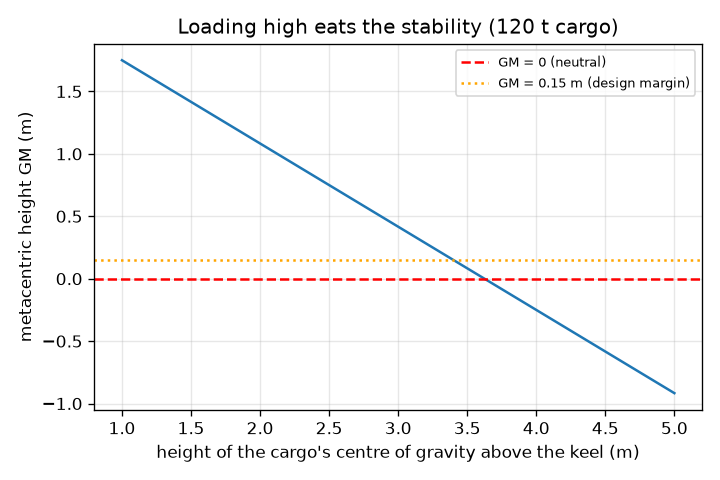
\includegraphics[width=0.85\linewidth]{figures/s03_gm_vs_height.png}\\\small Metacentric height against the height of the cargo's centre of gravity.\end{center}

\subsection*{E. Worked example}
The barge (20 x 6 x 2.5 m, empty 60 t with its centre of gravity 1.0 m above the keel) carries 120 t of cargo whose centre of gravity is 2.5 m above the keel, in fresh water. Find GM, and the righting arm at 10 degrees exactly and by the small-angle formula.
\begin{enumerate}[nosep]
\item Total mass 180 000 kg, so draft d = 180 000 / (1000 * 20 * 6) = 1.500 m.
\item KB = d / 2 = 0.750 m. BM = B\textasciicircum{}2 / (12 d) = 36 / 18 = 2.000 m. KM = 2.750 m.
\item KG = (60 * 1.0 + 120 * 2.5) / 180 = 360 / 180 = 2.000 m.
\item GM = 2.750 - 2.000 = 0.750 m, positive, so the barge rights itself.
\item Small angle at 10 degrees: GM sin(10 deg) = 0.750 * 0.1736 = 0.1302 m.
\item Wall-sided formula: sin(10 deg) (0.750 + 0.5 * 2.000 * tan\textasciicircum{}2(10 deg)) = 0.1736 * (0.750 + 0.0311) = 0.1356 m, which equals the exact numerical value 0.1356 m; the small-angle value is 4 percent low.
\end{enumerate}
\textbf{Answer.} GM = 0.750 m (stable). At 10 degrees the exact righting arm is 0.1356 m and the small-angle estimate is 0.1302 m.

\subsection*{F. Questions}
\begin{enumerate}[nosep]
\item \textbf{Conceptual.} A barge has 1.2 m of freeboard but capsizes when loaded with tall stacked cargo. Explain why freeboard does not guarantee stability, and what quantity does.
\item \textbf{Numerical.} The same barge carries 120 t with its centre of gravity at 3.0 m. Find KG and GM, and say whether it is stable.
\item \textbf{Graph and simulation interpretation.} From the GZ figure, at 20 degrees the exact curve is above the small-angle line. Read approximately both values for the loaded barge, state which is larger and give a likely reason for the difference.
\item \textbf{Design and optimisation challenge.} Design: with 160 t of cargo (instead of 120 t), find the highest cargo centre of gravity, in steps of 0.1 m, that keeps GM at or above 0.15 m. Compare it with the 3.40 m for 120 t and explain.
\end{enumerate}

\section{Real-world mini-project}
\textbf{How high can the deck cargo go?.} A barge 20 m long and 6 m wide (hull depth 2.5 m, empty mass 60 t, empty centre of gravity 1.0 m above the keel) will carry 120 t of cargo in fresh water. Two rules must hold: the metacentric height must be at least 0.15 m, and if the cargo slips 0.2 m sideways the barge must heel by no more than 10 degrees. Use \texttt{gm\_loaded} and \texttt{heel\_after\_shift} from Session 3 and find the highest cargo centre of gravity (in steps of 0.05 m) that meets each rule and both together.

\section{The path ahead}
\begin{enumerate}[nosep]
\item \textbf{Session 4: Free surface effect.} A barge model with a partly filled tank that reduces GM by its free-surface correction.
\item \textbf{Session 5: A round-bilge hull.} A generalised wet-section function for any polygon hull, with the GZ curve plotted.
\item \textbf{Session 6: Roll in time.} A time-stepping model of rolling that uses the GZ curve as the restoring moment.
\item \textbf{Session 7: Settle at the angle of loll.} A dynamic simulation of the failure case with a small disturbance.
\item \textbf{Session 8: A stability report for a loading plan.} A script that reads cargo items, finds KG, GM, the GZ curve and the area under it, and prints pass or fail.
\end{enumerate}

\section{Answers and hints}

\subsection*{Session 1}
\begin{enumerate}[nosep]
\item \textbf{Conceptual.} Hint: Think of the average density of the whole ship including the air inside. Solution: The ship is a hollow shell, so its total mass divided by its total outside volume (steel plus the air inside) is far below 1000 kg/m\textasciicircum{}3. In Python, a 150 kg steel boat of outside volume 0.8 m\textasciicircum{}3 has an average density of 187.5 kg/m\textasciicircum{}3 and floats, while the same 150 kg of steel as a lump has volume 0.019 m\textasciicircum{}3 and density 7850 kg/m\textasciicircum{}3 and sinks.
\item \textbf{Numerical.} Hint: Average density = mass / volume; compare with 1000. Solution: Density = 2.0 / 0.0030 = 666.7 kg/m\textasciicircum{}3, below 1000, so it floats. Fraction under water = 666.7 / 1000 = 0.667. It pushes aside 2.0 kg of water, the same as its own mass (check: 1000 * 0.0030 * 0.667 = 2.0 kg).
\item \textbf{Graph and simulation interpretation.} Hint: Find 1010 on the horizontal axis for each water and see whether the fraction reaches 1. Solution: In fresh water the fraction would be 1010 / 1000 = 1.01, which is more than 1, so it sinks. In sea water (1025) the fraction is 1010 / 1025 = 0.985, so it floats with 98.5 percent under water, just barely. Sea water gives a line that reaches 1 further to the right.
\item \textbf{Design and optimisation challenge.} Hint: Largest total mass = rho * A * draft\_max. Solution: Bottom area = 1.6 m\textasciicircum{}2. Largest total mass = 1000 * 1.6 * 0.25 = 400 kg, so the cargo is at most 400 - 150 = 250 kg. Assumptions: calm water, the boat stays upright, the cargo is spread evenly and the sides are tall enough. A real boat needs a bigger safety margin (waves, uneven loading), and Session 3 shows that stability can fail even when the boat floats.
\end{enumerate}

\subsection*{Session 2}
\begin{enumerate}[nosep]
\item \textbf{Conceptual.} Hint: Displaced water must weigh the same; compare the densities. Solution: The barge must displace the same mass of water, and sea water is denser, so the volume displaced is smaller and the draft decreases. The ratio is 1000 / 1025 = 0.976, so the draft drops by about 2.4 percent. It holds for any load, including the empty barge, because the rule is draft = m / (rho L B).
\item \textbf{Numerical.} Hint: draft = m / (rho L B) with rho = 1025. Solution: Draft = 160 000 / (1025 * 20 * 6) = 160 000 / 123 000 = 1.301 m, a little less than 1.333 m in fresh water. Check units: kg / (kg/m\textasciicircum{}3 * m * m) = m.
\item \textbf{Graph and simulation interpretation.} Hint: The deck line is at 2.5 m draft; solve m = rho L B H. Solution: Fresh water: 240 t; sea water: 1025 * 20 * 6 * 2.5 / 1000 - 60 = 247.5 t. The difference is 7.5 t, which is the extra 2.5 percent of displaced mass that denser water can support at the same volume.
\item \textbf{Design and optimisation challenge.} Hint: Capacity = rho * L * B * (H - f\_min) - raft mass, where raft mass = 10 * L * B. Solution: Capacity = 1000 * 3 * b * 0.15 - 30 * b = 420 b kg. For 15 people we need 975 kg, so b \textgreater{}= 975 / 420 = 2.32 m, and the narrowest width in steps of 0.1 m is 2.4 m (capacity 1008 kg, 15 people; at 2.3 m the capacity of 966 kg carries only 14). A wider raft gives a reserve for waves, uneven standing and heavier people, and it is also more stable (Session 3). The trade-off is more material, cost and weight to handle.
\end{enumerate}

\subsection*{Session 3}
\begin{enumerate}[nosep]
\item \textbf{Conceptual.} Hint: Compare the height of G with that of M. Solution: Freeboard says how far the deck is above the water; it comes from weight and buoyancy balancing (Session 2). Stability depends on where G is relative to M. Tall cargo raises G (KG) and lowers GM = KM - KG; if G rises above M, GM is negative and a small heel is pushed further by the water instead of being corrected, regardless of how much freeboard there is.
\item \textbf{Numerical.} Hint: KG = (60 * 1.0 + 120 * 3.0) / 180; KM is still 2.750 m. Solution: KG = (60 + 360) / 180 = 2.333 m. GM = 2.750 - 2.333 = 0.417 m. It is stable but with less than the 0.750 m of the worked example, and it is above the 0.15 m margin. Units: all heights in metres.
\item \textbf{Graph and simulation interpretation.} Hint: The deck edge goes under at 18.4 degrees; compare 0.298 and 0.257. Solution: At 20 degrees the exact GZ is 0.298 m and GM sin(phi) is 0.257 m: the exact curve is about 14 percent higher. The small-angle formula assumes the centre of buoyancy moves as if the waterplane stayed a rectangle; the BM tan\textasciicircum{}2(phi) term of the wall-sided formula adds the extra shift of B as the submerged shape becomes a wedge. By 20 degrees the deck edge is just under water, so even the wall-sided formula (0.302 m) starts to overestimate.
\item \textbf{Design and optimisation challenge.} Hint: Total 220 t gives draft 220 000 / 120 000 = 1.833 m; find KM and then KG\_max. Solution: Draft = 1.833 m, KB = 0.917 m, BM = 36 / (12 * 1.833) = 1.636 m, KM = 2.553 m. KG\_max = 2.553 - 0.15 = 2.403 m, so 60 + 160 h \textless{}= 2.403 * 220 = 528.7 and h \textless{}= 2.93 m; in steps of 0.1 m the answer is 2.9 m (GM = 0.171 m; at 3.0 m GM is 0.099 m, which fails). More cargo gives a lower height because it raises KG more and, since the draft rises, BM falls. Trade-off: carrying more means stowing it lower, e.g. in the hold, or accepting a smaller margin, which is not wise.
\end{enumerate}

\section{How to join}
Read \texttt{CONTRIBUTING.md} in the repository, then pick an issue labelled \texttt{good first issue}. Repository: \url{https://github.com/KrunalPanchal1995/openbuoyancy}

\end{document}
